\documentclass{article}

\usepackage{amsmath}
\usepackage{tikz}
\usetikzlibrary{bayesnet}

\renewcommand\phi\varphi

\begin{document}

Here is the derivation of Gibbs sampling for Model 1 of O'Connor 2013.
The model is adapted so that we consider all tuples with the same verb as coming
from the same ``document''.
This modification results in some simplification of the model (e.g. there are now
only $\phi$ distributions for subjects and objects as the verb argument is given).
Other than that it is intended to be the same...

Here is the generative story:

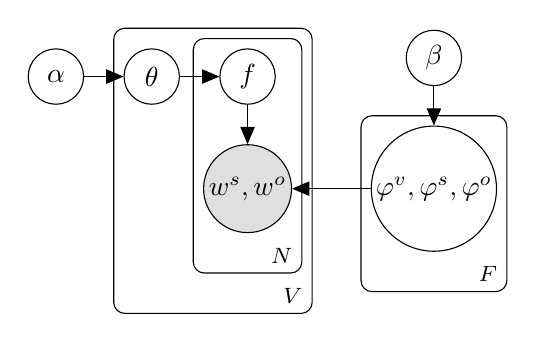
\begin{tikzpicture}[]
    \node[obs]                   (w)     {$w^s,w^o$}; %
    \node[latent, above=0.5cm of w]     (f)     {$f$};
    \node[latent, left=0.5cm of f]     (theta) {$\theta$};
    \node[latent, left=0.5cm of theta] (alpha) {$\alpha$};
    \node[latent, right=of w]    (phi)   {$\varphi^v,\varphi^s,\varphi^o$};
    \node[latent, above=0.5cm of phi] (beta) {$\beta$};
    \edge {alpha} {theta};
    \edge {theta} {f};
    \edge {f} {w};
    \edge {phi} {w};
    \edge {beta} {phi};
    \plate {frames} {(phi)} {$F$};
    \plate {datapoints} {(f) (w)} {$N$};
    \plate {verbs} {(f) (w) (datapoints) (theta)} {$V$};
\end{tikzpicture}


\begin{table}[h]
\begin{tabular}{ll}
$V$ & is the verb-vocabulary (equivallent to the number of documents)\\
$F$ & is the number of frames\\
$N^v$ & is the number of data points with verb $v$\\
$(w^s, w^o)^v_i$ & is data point $i$ (with verb (document) = $v$, subject = $w^s$ and object = $w^o$).\\
etc...\\
\end{tabular}
\end{table}

By the independence assumptions built into the model, we have:
\[
P(f,w,\theta,\phi|\alpha,\beta) = P(w|\phi,f) \cdot P(f|\theta) \cdot P(\theta|\alpha) \cdot P(\phi|\beta).
\]

Integrating out the latent distributions, we get:

\[
P(w,f|\alpha,\beta) = \int_\theta P(f|\theta)\cdot P(\theta|\alpha) d\theta \times
                      \int_\phi   P(w|f,\phi)\cdot P(\phi|\beta) d\phi
\]

First look at the first integral...

\begin{align*}
\int_{\theta} P(f|\theta)\cdot P(\theta|\alpha)\ d\theta
    =& \prod_{v=1}^V \int_{\theta^v} P(\theta^v|\alpha), P(f|\alpha)\ d\theta^v\\
    =& \prod_{v=1}^V \int_{\theta^v} P(\theta^v,f^v|\alpha)\ d\theta^v\\
    =& \prod_{v=1}^V DCM_\alpha(f^v)\\
    =& \frac{\Gamma(F\cdot\alpha)}{\Gamma(\alpha)^F} \times
       \frac{\prod_{f=1}^F\Gamma(C^v(f) + \alpha)}{\Gamma(F\cdot\alpha +
       \sum_{f=1}^FC^v(f))}
\end{align*}

Where $C^v(f)$ is the number data points with verb $v$ assigned to frame $f$.

The second integral is trickier, but we can still use DCM (I think?).

\begin{align*}
&\int_{\phi} P(w|f)\cdot P(\phi|\beta)\ d\phi\\
    =& \prod_{k=1}^F\int_{\phi^k} P(\phi^k|\beta)\cdot P(w[k]|f)\ d\phi^k\\
    =& \prod_{k=1}^F\int_{\phi^k_s} P(\phi^k_s|\beta)\cdot P(w_s[k]|f)\ d\phi^k_s
             \times \int_{\phi^k_o} P(\phi^k_o|\beta)\cdot P(w_o[k]|f)\ d\phi^k_o\\
\intertext{Where $w[k]$ is the sequence of data points consiering only those with frame assignment $k$
and $w_s[k]$ is the sequence of subjects from those data points.}
    =& \prod_{k=1}^F DCM_\beta(w_s[k]) \times DCM_\beta(w_o[k])\\
    =& \prod_{k=1}^F \frac{\Gamma(V^s\cdot\beta)}{\Gamma(\beta)^{V^s}}
              \times \frac{\prod_{s=1}^{V^s}\Gamma(C^{w[k]}(s) + \beta)}
                          {\Gamma(V^s\cdot\beta +\sum_{s=1}^{V^s}C^{w[k]}(s))}
              \times \frac{\Gamma(V^o\cdot\beta)}{\Gamma(\beta)^{V^o}}
              \times \frac{\prod_{o=1}^{V^o}\Gamma(C^{w[k]}(o) + \beta)}
                          {\Gamma(V^o\cdot\beta +\sum_{o=1}^{V^o}C^{w[k]}(o))}
\intertext{Where $C^{w[k]}(s)$ is the number of tuples with subject $s$ and frame $k$.}
\end{align*}

Next I want to find
\[
P(f_i = k| f_{-i}, w, \alpha, \beta) 
    = \frac{P(f_{-1}, f_i=k,w|\alpha,\beta)}
           {\sum_{k'=1}^F P(f_{-1}, f_i=k,w|\alpha,\beta)}
\]

This is where I am lost. I know that

\[
P(f,w|\alpha,\beta) = \prod_v^V DCM_\alpha(f^v)\times 
                      \prod_{k=1}^F DCM_\beta(W_s[k])\cdot DCM_\beta(w_o[k])
\]

But I'm not sure how to break this down into the conditional probabilities that I need.

\end{document}
